\chapter{Adapt to Frequent Network Failure and Limited Bandwidth}
%In this chapter, problems are further decomposed and analyzed. A variety of solutions are proposed and investigated. To prevent reinventing the wheel, enormous efforts have been put into studying existing technologies and tools in order to effectively solve the problem. 
It is important to formalize the problem and clarify what we attempt to achieve.

%Most of techniques today focus on reducing response time and improving concurrency, rather than offline operation and network partitioning. Even though major companies optimize their server architecture for miliseconds of faster, web service in rural areas is still a question of existance.

%TODO Read-only and Read-write

Overall goals are:
\begin{itemize}
\item To reduce user-perceived latency and bandwidth usage within the context of rural LAN with a narrow upper link.
\item To serve up-to-date content.
\item To achieve partition tolerance by continuing service when network failure occurs.
\end{itemize}

It has been proven that consistency, high availability and partition tolerence are impossible to be achieved at same time\cite{brewer2000towards}\cite{gilbert2002brewer}, however weak consistency is acceptable in our case. 

Since OUT online learning platform is already running in production phase, it is desired to impose minimum modifications to existing software stack.

\section{A closer look at Moodle} \label{components}
As introduced in section \ref{out_intro}, Moodle is deployed as underlying course management system for OUT E-learning platform. Moodle is an open sourse project written in PHP and well-documented\cite{aosamoodle}\cite{moodledoc}. Similiar to other web applications, it can be deployed in a typical LAMP or LNMP stack. In this chapter, we mainly focus on possible solutions for two problems stated previously, and leave the choice of actual server to chapter \ref{benchmark}

Moodle is a typical database-driven web application where all the pages are generated on-the-fly based on user request. The whole application is composed of three main components: 
\begin{itemize}
\item PHP source code, typically in \texttt{/var/www/moodle/}
\item A database to store data or metadata including site configuration, student information, course details, events, etc.
\item A directory to store materials and resources, as well as cache and temparory files. Typically it is named as \texttt{moodledata/}
\end{itemize}

As an online learning platform, interactive sessions cannot be neglected such as forum, quiz and user-generated blogs. Hence, modifications need to be preserved.
%TODO language

\section{Web Caching and Prefetching}
An intuitive and common solution for the problem of limited bandwidth is to cache popular web content locally, as illustrated in Figure \ref{with_cache}. Web caching has been proven as an effective approach to reduce bandwidth usage, user-perceived latency and loads on original server\cite{davison2001web}.

\begin{figure}[h]
\centering
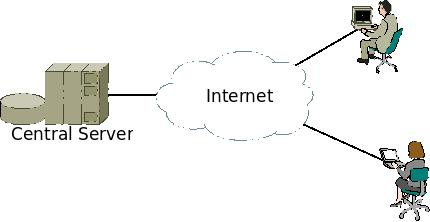
\includegraphics[width=0.6\textwidth]{../images/without_caching.jpeg}
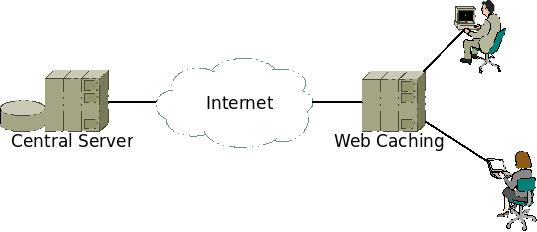
\includegraphics[width=0.6\textwidth]{../images/with_caching.jpeg}
\caption{Serve users without and with a Gateway Cache}
\label{with_cache}
\end{figure}

A proxy cache is normally a shared cache deployed in user network by administrator. It fetches Internet objects on the behalf of user and stores them locally. When next request for the same object arrives at proxy server, it responds with local copy and in turn reduces latency and saves bandwidth.

Although, two disadvantages are found when investigated against our case:
\begin{itemize}
\item Read-only Cache
Web cache proxy processes READ requests from users, whereas WRITE requests still go to original servers. Even though WRITE request can be evidently less than READ, they should still be satisfied during disconnections.
\item Cache Miss
Web cache proxy aims at accelarating web service, rather than replicating it. When cache miss occurs, users simply cannot access the service.
\end{itemize}

%One important feature of all web cache proxies is replacement strategy which invalidate caches and maintain freshness. A comprehensive survey of existing replacement strategy is presented in \cite{podlipnig2003survey}. However

\section{Content Delivery Network}
A Content Delivery Network is a collaborative set of surrogate servers spanning the network, where web contents are mirrored\cite{pathan2008content}. Users will perceive a smaller latency while fetching content from a nearby CDN surrogate server rather than original web server. The essence of CDN is illustrated in figure X
%TODO figure

Since more and more web services are evolving to provide dynamic content, CDN also takes advantages of cachebility hints when dealing with dynamic contents\cite{dilley2002globally}. 

%TODO open source CDN project


\section{Network File System}
A more brute-force approach is to replicate all three main components in section \ref{components} at local server and have all user requests redirected to it. As a standalone web service, a Moodle installation can be entirely replicated as long as those three components are copied and properly configured.

\subsection{Database Cluster}

\subsection{Database Replication and Synchronization}

\section{Multi-Master Database Synchronization}

\subsection{Concurrency Control Protocol}

\subsection{Operational Transformation}